\documentclass[11pt,twoside]{article}
%\documentclass[10pt,twoside,twocolumn]{article}
\usepackage[english]{babel}
\usepackage{times,subeqnarray}
\usepackage{url}
% following is for pdflatex vs. old(dvi) latex
\newif\myifpdf
\ifx\pdfoutput\undefined
%  \pdffalse           % we are not running PDFLaTeX
   \usepackage[dvips]{graphicx}
\else
   \pdfoutput=1        % we are running PDFLaTeX
%  \pdftrue
   \usepackage[pdftex]{graphicx}
\fi
\usepackage{apatitlepages}
% if you want to be more fully apa-style for submission, then use this
%\usepackage{setspace,psypub,ulem}
%\usepackage{setspace} % must come before psypub
%\usepackage{psypub}
\usepackage{psydraft}
%\usepackage{one-in-margins}  % use instead of psydraft for one-in-margs
%\usepackage{apa}       % apa must come last
\usepackage[natbibapa]{apacite}   % natbib
% \usepackage{csquotes}  % biblatex
% \usepackage[style=apa]{biblatex}
% \input netsym

% tell pdflatex to prefer .pdf files over .png files!!
\myifpdf
  \DeclareGraphicsExtensions{.pdf,.eps,.png,.jpg,.mps,.tif}
\fi

% use 0 for psypub format 
\parskip 2pt
% for double-spacing, determines spacing 
%\doublespacing
%\setstretch{1.7}

\columnsep .25in   % 3/8 in column separation

\def\myheading{ Correcting the Hebbian Mistake }

% no twoside for pure apa style, use \markright with heading only
\pagestyle{myheadings}
\markboth{\hspace{.5in} \myheading \hfill}{\hfill Zheng et al \hspace{.5in}}

\begin{document}
\bibliographystyle{apacite}

% sloppy is the way to go!
\sloppy
\raggedbottom

\def\mytitle{ Correcting the Hebbian Mistake: Toward a Fully Error-Driven Hippocampus }

\def\myauthor{Yicong Zheng, Xiaonan L. Liu, Satoru Nishiyama, Charan Ranganath, and Randall C. O'Reilly\\
  Departments of Psychology and Computer Science\\
  Center for Neuroscience\\
  University of California, Davis \\
  1544 Newton Ct\\
  Davis, CA 95616\\
  {\small oreilly@ucdavis.edu}\\}

\def\mynote{Draft Manuscript: Do not cite or quote without
  permission.\\

  R. C. O'Reilly is Chief Scientist at eCortex, Inc., which may derive indirect benefit from the work presented here.

  Supported by: ONR grants N00014-19-1-2684/ N00014-18-1-2116 (Deep learn), N00014-14-1-0670 / N00014-16-1-2128 (Bidir vis), N00014-18-C-2067 (MDM)

  This work utilized the Janus supercomputer, which is supported by the National Science Foundation (award number CNS-0821794) and the University of Colorado Boulder. The Janus supercomputer is a joint effort of the University of Colorado Boulder, the University of Colorado Denver and the National Center for Atmospheric Research.
}

\def\myabstract{
  The hippocampus plays a critical role in the rapid learning of new episodic memories. Many computational models propose that the hippocampus is an autoassociator that relies on Hebbian learning (i.e., “cells that fire together, wire together”). However, Hebbian learning is computationally suboptimal as it modifies weights unnecessarily beyond what is actually needed to achieve effective retrieval (“pattern completion”), causing more interference and resulting in a lower learning capacity. Our previous computational models have utilized a powerful, biologically plausible form of error-driven learning by contrasting local activity states at different points in time to create error signals in hippocampal CA1 (Ketz et al., 2013). New evidence regarding neurophysiological properties of the hippocampal subfield CA3 suggests that the hippocampus might be even more reliant on error-driven learning. Based on these findings, we propose a new model called Theremin (Total Hippocampal ERror MINimization) that incorporates biologically-based principles of error-driven learning in CA3, as well as CA1 as suggested by previous models. In the model, CA3 pyramidal cells respond to the entorhinal cortex (EC) monosynaptic input (EC$\rightarrow$CA3) prior to the EC disynaptic input through dentate gyrus (DG) (EC$\rightarrow$DG$\rightarrow$CA3). This signal delay gives rise to the temporal difference between the earlier EC-driven CA3 patterns and the later ones when DG inputs start to dominate, creating error signals to train the EC$\rightarrow$CA3 connection and CA3$\leftrightarrow$CA3 recurrent connection. In other words, DG serves as a teacher to CA3, correcting its patterns into more pattern-separated ones, thereby reducing interference. Results showed that Theremin, compared with our original model, has increasing model capacity and learning speed. Besides, activation dynamics in hippocampal subregions over the course of a learning trial and multiple interactions of learning illustrated how the error-driven learning environment contributes to better model performance. We close by presenting novel predictions from the model that can be tested in future studies.
}

% \titlesepage{\mytitle}{\myauthor}{\mynote}{\myabstract}
% \twocolumn

%\titlesamepage{\mytitle}{\myauthor}{\mynote}{\myabstract}

\titlesamepageoc{\mytitle}{\myauthor}{\mynote}{\myabstract}

% single-spaced table of contents, delete if unwanted
% \newpage
% \begingroup
% \parskip 0em
% \tableofcontents
% \endgroup
% \newpage

% \twocolumn

\pagestyle{myheadings}

\section{Introduction}

It is well-established that the hippocampus plays a critical role in the rapid learning of new episodic memories \citep{EichenbaumYonelinasRanganath07}.  Most computational and conceptual models of this hippocampal function are based on principles first articulated by Donald O. Hebb and David Marr \citep{Hebb49,Marr71,McNaughtonNadel90,McClellandMcNaughtonOReilly95}.  At the core of this framework is the notion that recurrent connections among CA3 neurons are strengthened when they are co-activated (``cells that fire together, wire together''), essentially creating a cell assembly of interconnected neurons that bind the different elements of an event.  As a result of this Hebbian learning, subsequent partial cues can drive pattern completion to recall the entire original memory, by reactivating the entire cell assembly via the strengthened interconnections.

In addition, Marr's fundamental insight was that sparse levels of neural activity in area CA3, and especially the large numbers of largely silent dentate gyrus (DG) granule cells, will drive the creation of cell assemblies that involve a distinct combination of neurons for each event, otherwise known as \emph{pattern separation} \citep{Marr71,OReillyMcClelland94,YassaStark11}.  As a consequence, the DG to CA3 pathway has the capability to minimize interference from learning across even closely overlapping episodes (e.g., where you parked your car today vs. where you parked it yesterday).  Overall, the basic tenets established by Hebb and Marr account for a vast amount of behavioral and neural data on hippocampal function, and is as close to a ``settled theory'' as any in neuroscience \citep{OReillyBhattacharyyaHowardEtAl14,YonelinasRanganathEkstromEtAl19,MORE}.
 
Although almost every biologically-based computational model of hippocampal function incorporates Hebbian plasticity, it is notable that Hebbian learning is computationally suboptimal in various respects, especially in terms of overall learning capacity \citep{Abu-MostafaSt.Jacques85,TrevesRolls91}.  In models that rely solely on Hebbian learning, whenever two neurons are active together, the synaptic weight between them is increased, regardless of how necessary that change might be to achieve better memory recall.  As a result, such models do not know when to stop learning, and continue to drive synaptic changes beyond what is actually necessary to achieve effective pattern completion.  The consequence of this ``learning overkill'' is that all those unnecessary synaptic weight changes end up driving more interference with the weights needed to recall other memories, significantly reducing overall memory capacity. Even the high degree of pattern separation in the DG to CA3 pathway is not sufficient to make up for the interference caused by reliance on Hebbian learning. 

One logical alternative to the simple Hebbian approach is to introduce a self-limiting learning mechanism that drives only synaptic changes that are absolutely necessary to support learning.  However, determining this minimal amount of learning can be challenging: how can local synaptic changes ``know'' what is functionally necessary in terms of the overall memory system function?  One well-established class of such learning mechanisms are error-driven learning rules: by driving synaptic changes directly in proportion to a functionally-defined error signal, learning automatically stops when that error signal goes to zero. For example, the well-known Rescorla-Wagner learning rule for classical conditioning \citep{RescorlaWagner72} is an instance of the delta-rule error-driven learning rule \citep{WidrowHoff60}:
\begin{equation}
	dW = x (r - y),
\end{equation}
where $dW$ is the amount of synaptic weight change, $x$ is the sending neuron activity level (e.g., average firing rate of sensory inputs representing conditioned stimuli), $r$ is the actual amount of reward received, and $y$ is the expected amount of reward, computed according to the existing synaptic weights:
\begin{equation}
	y = \sum x W.
\end{equation}

This learning rule drives learning (changes in weights, $dW$) up to the point where the expected prediction of reward ($y$) matches the actual reward received ($r$), at which point learning stops, because the difference term in the parentheses goes to 0. The dependency on $x$ is critical for \emph{credit assignment}, which ensures that the most active sending neurons change their weights the most, as such weight changes will be the most effective in reducing the error.  The widely-used error backpropagation learning algorithm is a mathematical extension of this simpler delta-rule form of learning \citep{RumelhartHintonWilliams86}, and demonstrates the general-purpose power of these error-driven learning principles \citep{LeCunBengioHinton15}.

To be able to apply a similar self-limiting error-driven learning computation to the hippocampus, we need a target signal that determines when the learning has accomplished what it needs to do, to achieve the overall memory functionality required.  What kind of natural target signal is there for the hippocampus?  Hippocampal episodic encoding is widely regarded as automatically, continuously, and rapidly storing new memories as they occur in real time, which seems more like a Hebbian form of learning as compared to error-driven learning.  Nevertheless, we have previously shown that error-driven learning principles can be applied to the CA1 region of the hippocampus \citep{KetzMorkondaOReilly13}, building on theta-phase dynamics discovered by \citet{HasselmoBodelonWyble02}.  These error-driven learning dynamics have been supported by studies of CA1 learning \citep{SchapiroTurk-BrowneNormanEtAl16,SchapiroTurk-BrowneBotvinickEtAl17}.

Building upon this prior work, and a recent proposal by \citet{KowadloAhmedRawlinson20}, we extend the application of error-driven learning to the ``heart'' of the hippocampus: learning in the feedforward and recurrent synapses of area CA3.  The key idea is that the DG can serve as a teacher to the CA3, driving learning just to the point where CA3 on its own can replicate the same highly pattern-separated representations that the DG imparts on the CA3.  We show that this more fully error-driven hippocampal learning system has significantly improved memory capacity and resistance to interference compared to one with Hebbian learning in CA3.  Furthermore, we show how these error-driven learning dynamics fit with detailed features of the neuroanatomy and physiology of the hippocampal circuits, and can have broad implications for understanding important learning phenomena such as the testing effect \citep{LiuEtAl21}.  Overall, this new framework provides a consistent computational and biological account of hippocampal episodic learning, which departs from the tradition of Hebbian learning at a computational level, while retaining the overall conceptual understanding of the essential role of the hippocampus in episodic memory.

In the remainder of the paper, we first introduce the computational and biological framework for error-driven learning in the hippocampal circuits, and then present the details of an implemented computational model, followed by results of this model as compared to our previous Hebbian-CA3 version \citep{KetzMorkondaOReilly13}, as well as representational analyses that capture the subregional dynamics in the model.  We conclude with a general discussion, including testable predictions from this framework and implications for some salient existing behavioral and neural data on hippocampal learning.

\section{Sources of Error Driven Learning in the Hippocampal Circuit}

\begin{figure}
  \centering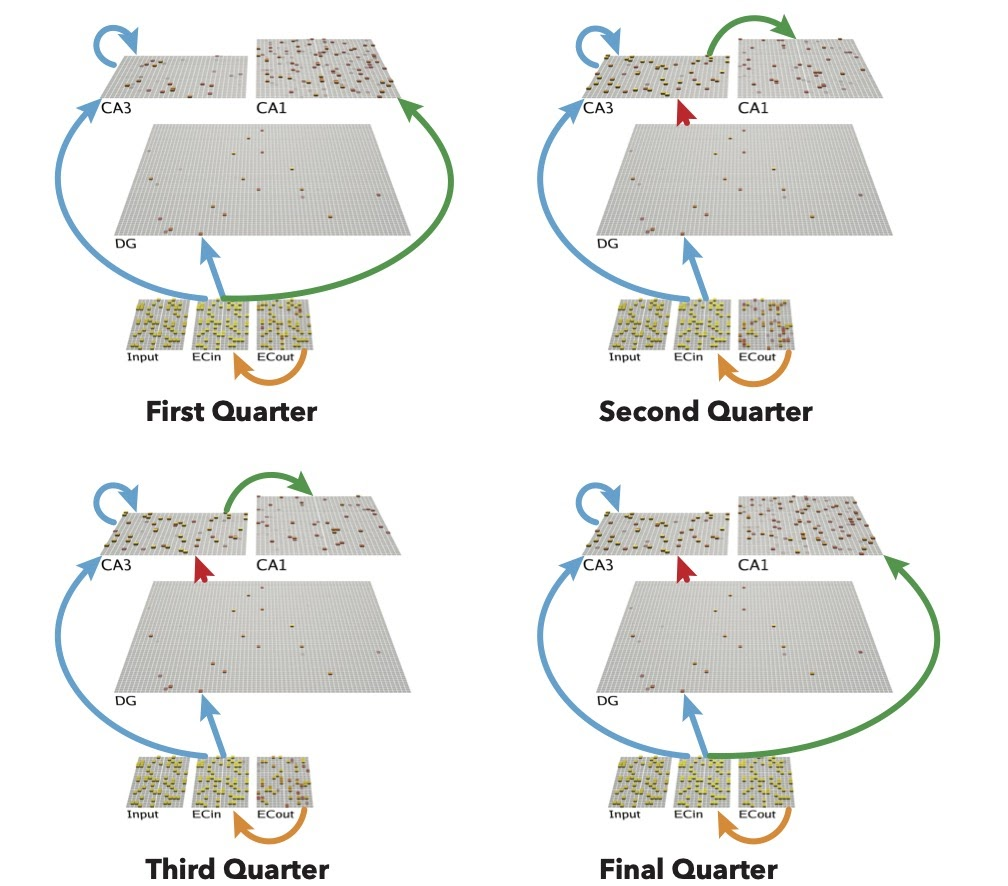
\includegraphics[width=4in]{fig_hip_edl_model}
  \caption{\footnotesize Architecture of the Theremin model. Visual depiction of one full training trial in Theremin, separated by four different sequential time points (i.e., four quarters). Arrows depict theoretically important weight modifications in that quarter; on the contrary, connections not implied by arrows did not change their weights. Blue and red arrows indicate the new CA3 dynamics in CA3, with red arrows sourcing into CA3 after the first quarter and create temporal difference error signals. Green arrows indicate the theta-phase \citep{KetzMorkondaOReilly13} dynamics in CA1. Orange arrows indicate hippocampal output EC signals that get sent back into the hippocampal network (i.e., big-loop signals).}
\label{fig.theremin}
\end{figure}

We begin by briefly reviewing our earlier work showing how the monosynaptic pathway interconnecting the entorhinal cortex (EC) and area CA1 can support error-driven learning, via systematic changes in pathway strengths across the theta cycle \citep{KetzMorkondaOReilly13,HasselmoBodelonWyble02} (Figure~\ref{fig.theremin}).  Although nominally a central part of the hippocampus, from a computational perspective it makes more sense to think of this monosynaptic CA1 $\leftrightarrow$ EC pathway (sometimes known as the temporo-ammonic pathway) as an extension of the neocortex, where the principles of error-driven learning have been well-developed \citep{OReilly96,WhittingtonBogacz19}.  Specifically, this pathway can be thought of as learning to encode the EC information in CA1 in a way that can then support reactivation of the corresponding EC activity patterns when memories are later retrieved via CA3 pattern completion.  Computationally, this is known as an \emph{auto-encoder}, and error-driven learning in this case amounts to adjusting the synapses in this monosynaptic pathway to ensure that the EC pattern is accurately reconstructed from the CA1 activity pattern.

Using the delta rule equation shown above, this objective can be formulated as:
\begin{equation}
dW = \mbox{CA1} (\mbox{ECin} - \mbox{ECout}),
\end{equation}
where \emph{ECin} is the EC input pattern driven by cortical inputs to the EC, and \emph{ECout} is the output produced by the CA1 encoding of this ECin pattern (Figure~\ref{fig.theremin}).  If these are identical, then the error is 0, and no learning occurs, and any learning that does occur is directly in proportion to the extent of error correction required.  The detailed biological story for how the system could implement this error-driven learning mechanism depends on the relative out-of-phase strengths of the two major projections into the CA1 \citep{HasselmoBodelonWyble02}: in one phase the CA1 is driven more strongly by direct ECin layer 3 inputs, and in another it is driven more by the CA3 projections.  Furthermore, the ECout (deep layers) is initially driven by CA1, but then is driven more by ECin (layer 3).

The net effect is that, by learning based on temporal differences in activation state over time, the delta rule is realized.  Specifically, the difference in ECout activation between their CA1-driven vs. ECin-driven states produces the (ECin - ECout) difference in the above equation.  Likewise, CA1 neurons directly experience a ``reflection'' of this temporal difference, conveyed via the projections from ECout $\rightarrow$ CA1, and they also can learn using their own local delta-rule-like equation based on this temporal difference.  Mathematically, this is a form of error backpropagation \citep{OReilly96,WhittingtonBogacz19}, which is more properly the version of error-driven learning powering modern deep networks.  See \citet{KetzMorkondaOReilly13} for more details.  Consistent with the idea that this monosynaptic pathway is more cortex-like in nature, \citet{SchapiroTurk-BrowneBotvinickEtAl17} have shown that this pathway can learn to integrate across multiple learning experiences to encode sequential structure, in a way that depends critically on the error-driven nature of this pathway, and is compatible with multiple sources of data \citep{SchapiroTurk-BrowneNormanEtAl16}.

In this paper, we extend error-driven learning principles to the remainder of the hippocampal system, showing how the main trisynaptic pathway involving the EC, DG, and CA3 can support error-driven learning, resulting in dramatic improvements in overall learning capacity.  As a result of an extensive parameter search with these new mechanisms, we discovered a few other important principles that enhance episodic learning performance as well.

The primary challenge in extending error-driven learning to the trisynaptic pathway is in deriving an error signal that drives learning toward effective memory encoding.  As captured in the delta rule equation, the essential ingredient is to have two different states, one that represents a better, target representation (e.g., the actual reward, or the actual ECin input in the examples considered previously) that can be compared against what the current synaptic weights produce on their own, so that these weights can be adjusted to better achieve the target representation.  In this framing, one can consider the highly pattern-separated activity pattern in the DG, to provide a kind of target representation relative to what the CA3 can produce on its own (i.e., prior to the arrival of DG $\rightarrow$ CA3 inputs).  Thus, in effect, the DG is serving as a teacher to the CA3, driving error-driven learning signals there just to the point where CA3 on its own can replicate the DG-driven sparse, pattern-separated representations \citep{KowadloAhmedRawlinson20}.

The delta-rule formulation for this new error-driven learning component is:
\begin{equation}
dW = \mbox{ECin} (\mbox{CA3}_{dg} - \mbox{CA3}_{nodg}),
\end{equation}
where \emph{ECin} is the sending activity into CA3 (via the perforant pathway (PP) projections), $\mbox{CA3}_{dg}$ is the activity of the CA3 neurons when being driven by the strong mossy fiber (MF) inputs from the DG, and $\mbox{CA3}_{nodg}$ is the CA3 activity when not being driven by those DG inputs, i.e., from only the PP and CA3 recurrent inputs prior to the arrival of DG $\rightarrow$ CA3 inputs.  In this way, the DG, which is the sparsest and most pattern-separated hippocampal layer, is serving as an error-driven teacher to CA3, teaching it to adopt its highly pattern-separated view of the input pattern.  Critically, to the extent that CA3 is already matching the DG pattern separation, no additional learning needs to occur, thus producing the interference minimization benefits of error-driven learning.  Note that the same error-driven signal in CA3 trains the lateral recurrent pathway within CA3 in addition to the ECin $\rightarrow$ CA3 PP projections, so that these recurrent connections also adapt to fit the DG-driven pattern, but no further.

Although this form of error-driven learning may make sense computationally, how could something like this delta error signal emerge naturally from the hippocampal biology?  First, as in our prior model of learning in the monosynaptic pathway \citep{KetzMorkondaOReilly13}, we adopt the idea that the delta arises as a \emph{temporal difference} between two states of activity over the CA3 (which is also consistent with a broader understanding of how error-driven learning works in the neocortex; \citep{OReilly96,OReillyMunakata00,OReillyRussinZolfagharEtAl21}). The appropriate temporal difference over CA3 should actually emerge naturally from the additional delay associated with the propagation of the MF signal through the DG to the CA3, compared to the more direct PP signal from ECin to CA3.  Thus, as in our prior models, the minus phase term in the delta rule occurs first (i.e., $\mbox{CA3}_{nodg}$), followed by the plus phase (this terminology goes back to the Boltzmann machine, which also used a temporal-difference error-driven learning mechanism; \citealp{AckleyHintonSejnowski85}).

Neurophysiologically, there are a number of lines of empirical evidence consistent with this temporal difference error-driven learning dynamic in the CA3:
\begin{itemize}

	\item CA3 pyramidal cells respond to PP stimulation prior to the granule cells (GCs) in the DG, in vivo \citep{YeckelBerger90,DoMartinezMartinezEtAl02}, such that the indirect input through the DG will be that much more delayed due to the slower DG response (by roughly 5 msec at least).

    \item MF inputs from the DG GCs to the CA3 can induce heterosynaptic plasticity at PP and CA3 recurrent connections \citep{McMahonBarrionuevo02,TsukamotoYasuiYamadaEtAl03,KobayashiPoo04,RebolaCartaMulle17}. This is consistent with ability of the later-arriving DG inputs to drive the CA3 synaptic changes toward that imposed by this stronger target-like pattern, compared to the earlier pattern initially evoked by PP and CA3 recurrent inputs.

    \item Although several studies have found that contextual fear learning is intact without MF input to CA3 \citep{McHughJonesQuinnEtAl07,NakashibaCushmanPelkeyEtAl12,KitamuraSunMartinEtAl15}, incomplete patterns from DG during encoding impair the function of EC $\rightarrow$ CA3 pathway in contextual fear conditioning tasks \citep{BernierLacagninaAyoubEtAl17}, suggesting that DG still plays an important role in heterosynaptic plasticity at CA3.
\end{itemize}

In addition to this DG-driven error learning in CA3, we explored a few other important principles that also help improve overall learning performance.  First, reducing the strength of the MF inputs to the CA3 during memory recall helped shift the dynamics toward pattern completion instead of pattern separation, as was hypothesized in \citet{OReillyMcClelland94}.  This is consistent with evidence showing that MF projections are not necessary in naturally recalling a memory \citep{NakashibaCushmanPelkeyEtAl12,BernierLacagninaAyoubEtAl17}.  However, other data suggests that it still plays an important role in increasing recall precision \citep{RuedigerVittoriBednarekEtAl11,NakashibaCushmanPelkeyEtAl12,BernierLacagninaAyoubEtAl17,PignatelliRyanRoyEtAl19}. Thus, consistent with these data, we found that reducing, but not entirely eliminating MF input to the CA3 during recall was beneficial, most likely because it enabled the other pathways to exert a somewhat stronger influence in favor of pattern completion, while still preserving the informative inputs from the DG.

Second, we experimented with the parameters on the one remaining Hebbian form of learning in the network, which is in the ECin $\rightarrow$ DG pathway.  This pathway does not have an obvious source of error-driven contrast, given that there is only one set of projections into the DG granule cells.  In effect, the DG serves as a teacher to the CA3, so what is left over to teach the teacher itself?  Thus, we sought to determine if there were particular parameterizations of Hebbian learning that would optimize learning in this pathway, and found that shifting the balance of weight decreases over weight increases helped learning overall, working to increase pattern separation in this pathway still further.

Finally, we tested a range of different learning rates for all of the pathways in the model, along with relative strengths of the projections, across a wide range of network sizes and numbers of training items, to determine the overall best parameterization under these new mechanisms.

Next, we describe our computational implementation within the existing \citet{KetzMorkondaOReilly13} framework, and then present the results of a systematic large-scale parameter search of all relevant parameters in the model, to determine the overall best-performing configuration of the new model. 

\section{Methods}

\subsection{Hippocampal Architecture}

The current model, which we refer to as the Theremin (colorfully capturing the concept of Total Hippocampal ERror MINimization)(Figure~\ref{fig.theremin}), is based on our previous theta-phase hippocampus model \citep{KetzMorkondaOReilly13}, which was developed within the earlier Complementary Learning System (CLS) model of the hippocampus \citep{NormanOReilly03,OReillyRudy01}.  The broader implementation framework is the Leabra model (Local, Error-driven, and Associative, Biologically Realistic Algorithm), which provides standard point-neuron rate-coded neurons, inhibitory interneuron-mediated competition and sparse, distributed representations, full bidirectional connectivity, and temporal-difference based error-driven learning dynamics \citep{OReillyMunakata00,OReillyMunakataFrankEtAl12}.  See \url{https://github.com/emer/leabra} for fully-documented equations, code, and several example simulations, including the exact model presented here.

Figure~\ref{fig.theremin} shows the standard hippocampal architecture captured in our models. The EC superficial layer (ECin) is the source of input to the hippocampus, integrated from all over the cortex.  Based on anatomical and physiological data, we organize the EC into different pools (also called slots) that reflect the inputs from different cortical areas, and thus have different types of representations reflecting the specializations of these different areas \citep{WitterDoanJacobsenEtAl17}.  In the present model, we assume some pools reflect item-specific information, while others reflect the various aspects of information that together constitute context, which is important for distinguishing different memory lists in our tests.

The ECin projects to the Dentate Gyrus (DG) and CA3 via broad, diffuse PP projections, which have a uniform 25\% random chance of connection.  This connectivity is essential for driving conjunctive encoding in the DG and CA3, such that each receiving neuron receives a random sample of information across the full spectrum present in the ECin.  Further, the DG and CA3 have high levels of inhibition, driving extreme competition, such that only those neurons that have a particularly favorable conjunction of input features are able to get active in the face of the strong inhibition.  This is the core principle behind Marr's pattern separation mechanism, captured by his simple R-theta codon model \citep{Marr71}.  Using the standard FFFB (feedforward \& feedback) inhibition mechanism in Leabra, DG has a inhibitory conductance multiplier of 3.8 and CA3 has 2.8, compared to the standard cortical value of 1.8 which produces activity levels of around 15\%.  These resulted in DG activity around 1\% and CA3 around 2\%.

The CA3 receives strong MF projections from the DG, which have a strength multiplier of 4 (during encoding), giving the DG a much stronger influence on CA3 activity compared to the direct PP inputs from ECin.  CA3 also receives recurrent collateral projections which have a strength multiplier of 2, which are the critical Hebbian cell-assembly autoassociation projections in the standard Hebb-Marr model, as captured in \cite{KetzMorkondaOReilly13} using a Hebbian learning mechanism.  That model also uses Hebbian learning in the PP pathways from ECin to DG and CA3, which also facilitate pattern completion during recall as analyzed in \citet{OReillyMcClelland94}.

In the monosynaptic pathway, ECin (superficial) layers project to CA1, which then projects back into the deep layers of EC, called ECout in the model, such that CA1 encodes the information in ECin and can drive ECout during recall to drive the hippocampal memory back out into the cortex.  This is the auto-encoder function of CA1, which is essential for translating the highly pattern-separated representations in CA3 back into the ``language'' of the cortex.  Thus, a critical locus of memory encoding is in the CA3 $\rightarrow$ CA1 connections that associate the CA3 conjunctive memory with the CA1 decoding thereof --- without this, the randomized CA3 patterns would be effectively unintelligible to the cortex.

Unlike the broad and diffuse PP projections, the EC $\leftrightarrow$ CA1 connections obey the pool-wise organization of EC, consistent with the focal, point-to-point nature of the EC $\leftrightarrow$ CA1 projections \citep{WitterDoanJacobsenEtAl17}.  Thus, each pool is separately auto-encoding the specific, specialized information associated with a given cortical area, which enables these connections to slowly learn the systematic ``language'' of that area.  The entire episodic memory is thus the distributed pattern across all of these pools, but the monosynaptic pathway only sees a systematic subset, which it can efficiently and systematically auto-encode.

The purpose of the theta-phase error-driven learning in the \citet{KetzMorkondaOReilly13} model is to shape these synaptic weights to support this systematic auto-encoding of information within the monosynaptic pathway.  Specifically, CA1 patterns at peaks and troughs of theta cycles come from CA3-retrieved memory and ECin inputs, respectively.  As shown in equation 3 above, the target plus-phase activation comes from the ECout being strongly driven by the ECin superficial patterns, in contrast to the minus phase where ECout is being driven directly by CA1.  Thus, over iterations of learning, this error-driven mechanism shapes synapses so that the CA1 projection to ECout will replicate the corresponding pattern on ECin.

Relative to this theta-phase model, the new Theremin model introduces error-driven learning in the CA3, using equation 4 as shown above, which was achieved by delaying the output of DG $\rightarrow$ CA3 until the 2nd theta phase cycle (Figure~\ref{fig.theremin}).  Thus, the plus phase represents the CA3 activity in the presence of these strong DG inputs, while the minus phase is the activity prior to the activation of these inputs.  In addition, as noted earlier, we tested the effects of reducing the strength of MF inputs to CA3 during recall testing, along with testing all other relevant parameters in a massive grid search.

\subsection{Model Testing}

\begin{figure}
  \centering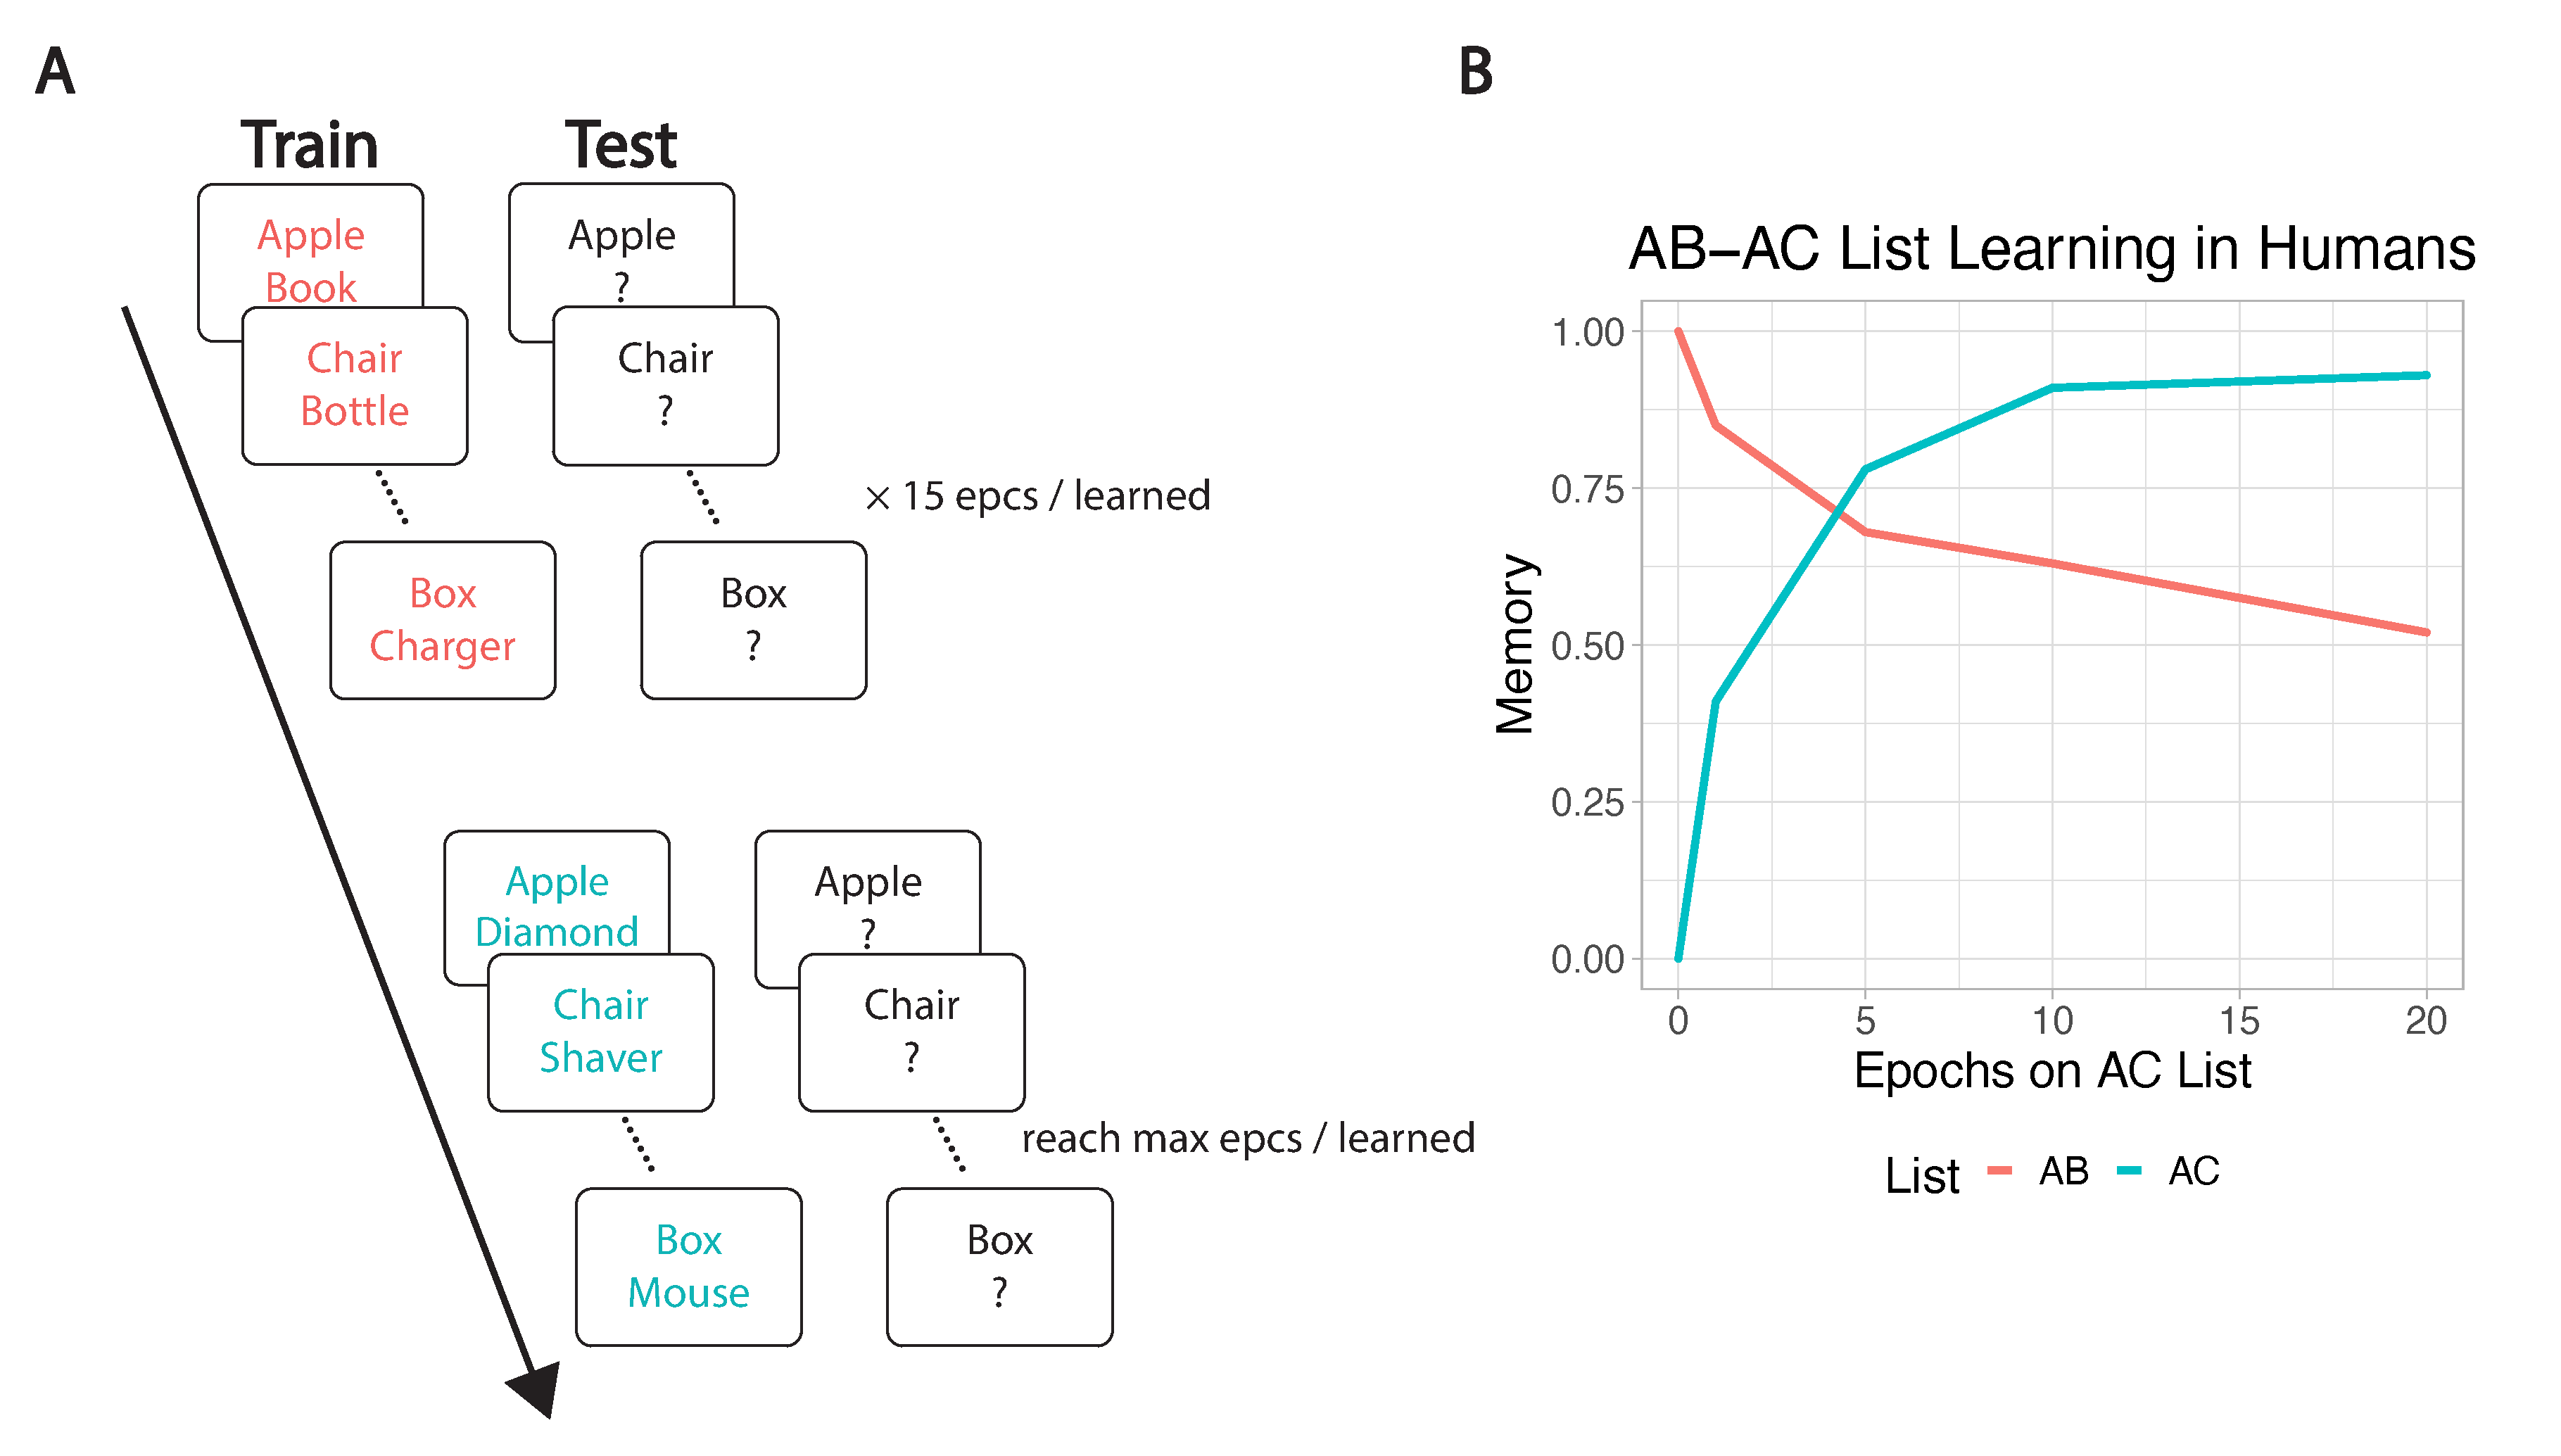
\includegraphics[width=4in]{fig_hip_edl_abac}
  \caption{\footnotesize ABAC list learning paradigm diagram and human data reproduced from an empirical experiment \citep{BarnesUnderwood60}. A) Depicted in the diagram is the ABAC list learning task used in the current study. The first ``learned'' means AB memory reaches 100\%; the second ``learned'' means AC memory reaches 100\%. The maximum number of epochs in the task is 30. Detailed procedure is described in Materials \& Method. B) Human participants showed moderate interference of the AB list after learning the AC list. Note that there were 20 epochs following AC list learning in the original human experiment, unlike the current task design. }
\label{fig.abac}
\end{figure}

The task used in the current study is a standard AB-AC paired-associates list-learning paradigm, widely used to stress interference effects \citep{BarnesUnderwood60,McCloskeyCohen89} (Figure~\ref{fig.abac}). In these paradigms, typically, a participant learns a list of word pairs, with each pair referred to as \emph{A-B}. Once the pairs are learned to a criterion or a fixed number of repetitions, participants learn a new list of \emph{A-C} word pairs, in which the first word in each \emph{A-B} pair is now associated with a new word. Learning of A-C pairs is typically slowed due to competition with previously learned A-B pairs (\emph{proactive interference}), and once the A-C pairs are learned, retention of A-B pairs is reduced (\emph{retroactive interference}).

To simulate the AB/AC paradigm, each pair of A and B items (unique random bit patterns in the model) was trained, and then tested by probing with the A item and testing for recall of the associated B item.  A list context representation was also present during training and testing, to distinguish the AB vs. AC list.  Once recall accuracy for all AB pairs reached 100\%, or 15 epochs of the whole AB list have been trained, the model switched to learn the AC list, where previously learned A items were paired with novel C items and AC list context. Similarly, if memory for all AC pairs reached 1, or 30 epochs have been trained in total, that run was considered complete.  We ran 30 different simulated subjects (i.e., runs) on each configuration and set of parameters, with each such subject having a different set of random initial synaptic weights. 

There are several central questions that we address in turn.  First, we compared the earlier theta-phase hippocampus model with the new Theremin model to determine the overall improvement resulting from the new error-driven learning mechanism and other optimized parameters.  This provides an overall sense of the importance of these mechanisms for episodic memory performance, and an indication of what kinds of problems can now be solved using these models, at a practical level.  In short, the Theremin model can be expected to perform quite well learning challenging, overlapping patterns, opening up significant new practical applications of the model.

Next, we tested different parameterizations of the Theremin model, to determine the specific contributions of: 1) error-driven learning specifically in the CA3, compared to Hebbian learning in this pathway, with everything else the same; 2) reduced MF strength during testing (cued recall); 3) the balance of weight decreases vs. increases in the ECin $\rightarrow$ DG projections; 4) the effect of pretraining on the monosynaptic pathway between EC and CA1, which simulates the accumulated learning in CA1 about the semantics of EC representations, reflecting in turn the slower learning of cortical representations. In other words, human participants have extensive real life experience of knowing the A/B/C list items, enabling the CA1 to already be able to invertably reconstruct the corresponding EC patterns for them, and pretraining captures this prior learning.  Pretraining has relatively moderate benefits for the Theremin model, and was used by default outside of this specific test.  The pretraining process involved turning DG and CA3 off, while training the model with items and context separately only in the monosynaptic EC $\leftrightarrow$ CA1 pathway for 5 epochs. 

The learning capacity of a model is proportional to its size, so we tested a set of three network sizes (small, medium, large) to determine the relationship between size and capacity in each case.  The list sizes ranged from 20 to 100 pairs of AB/AC associations (\citet{BarnesUnderwood60} used 8 pairs of nonsense syllables). It is worth noting that the number of units in DG is roughly 5 times to that in CA3, consistent with the theta-phase hippocampus model.

For the basic performance tests, the two dependent variables were NEpochs and ABmem.  NEpochs measures the total number of epochs used to finish one full run through AB and AC lists, which measures the overall speed of learning (capped at 30 if the network failed to learn). ABmem is the memory for AB pairs after learning the AC list, thus representing the models' ability to resist interference.

In addition to these performance tests, we ran representational analyses on different network layers (i.e., hippocampal subregions) over the course of learning.  This enabled us to directly measure the temporal difference error signals that drove learning in Theremin, and how representations evolved through learning.  Furthermore, by comparing across differences in learning algorithm and other parameters, we can directly understand the overall performance differences.  The main analytic tool here is to compute cycle-by-cycle correlations between the activity patterns present at that cycle, and the patterns present at the end of a trial of processing (100 cycles), which provides a simple 1-dimensional summary of the high-dimensional layer activation patterns as they evolve over time.

\section{Results}

\subsection{Overall memory performance}

\begin{figure}
  \centering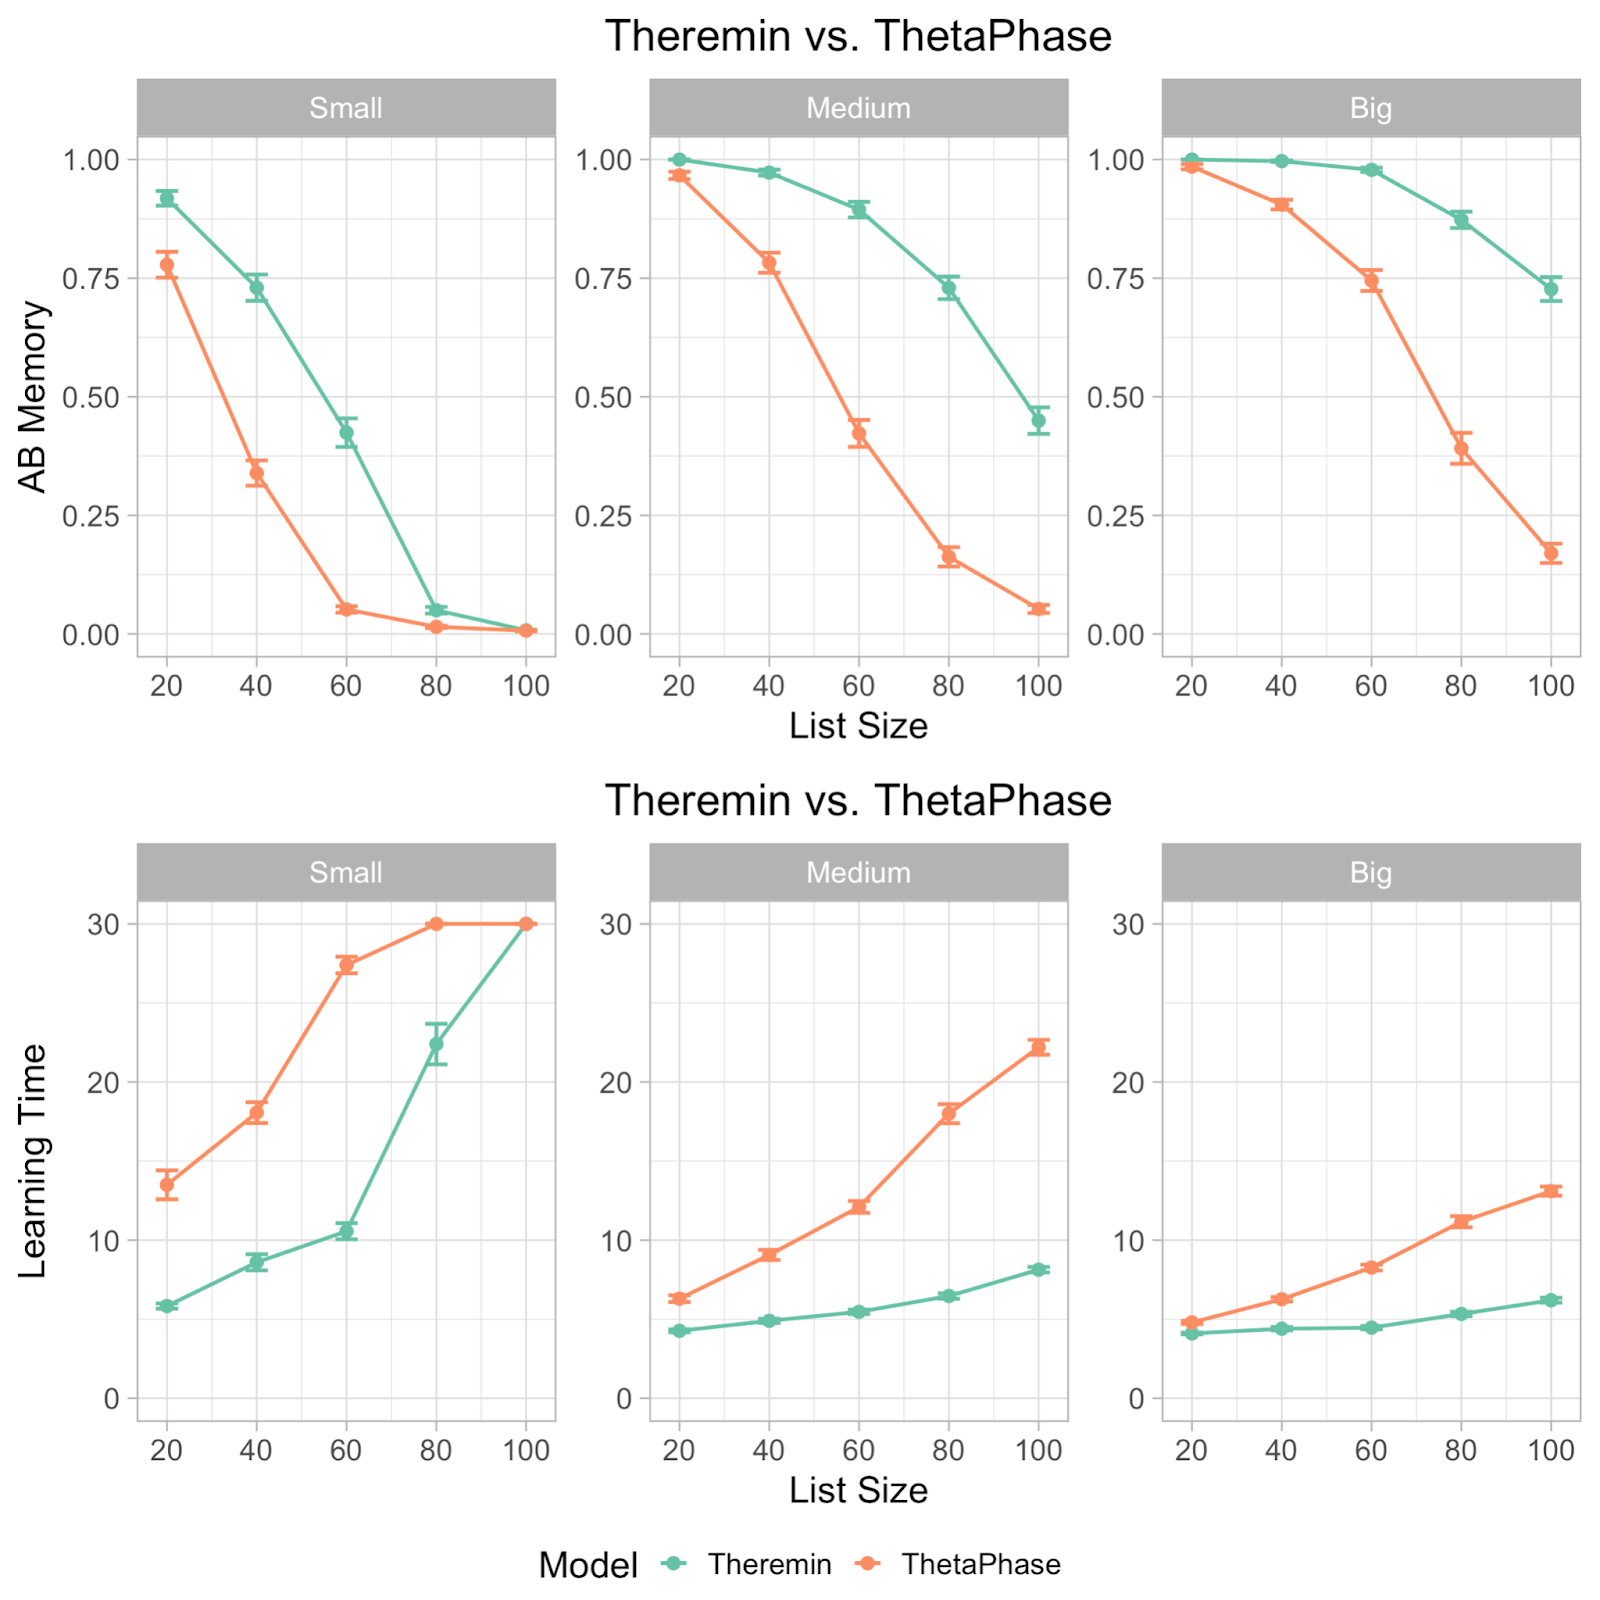
\includegraphics[width=4in]{fig_hip_edl_thetaphase}
  \caption{\footnotesize Theremin vs. ThetaPhase on AB memory and learning time for all three network sizes, the full Theremin had significantly faster  training time across all list sizes and network sizes.  Likewise, Theremin was better at counteracting interference across all list sizes and network sizes.}
\label{fig.thetaphase}
\end{figure}

First, we examined the broadest measure of overall learning performance improvements in Theremin compared to the earlier theta-phase model.  Figure~\ref{fig.thetaphase} shows the results across all three network sizes and numbers of list items.  For all three network sizes, the ABmem results show that Theremin was better at counteracting interference and retained more memory for AB pairs than the theta-phase hippocampus model across all list sizes and network sizes (\emph{ps} \textless \ .01 except SmallHip List100 (\emph{p} = 0.736)). Moreover, the full Theremin model completed learning significantly faster (i.e., the NEpochs measure) than the theta-phase hippocampus model across all list sizes and network sizes (\emph{ps} \textless \ .01 except SmallHip List100 (all NEpochs = 30)).

\begin{figure}
  \centering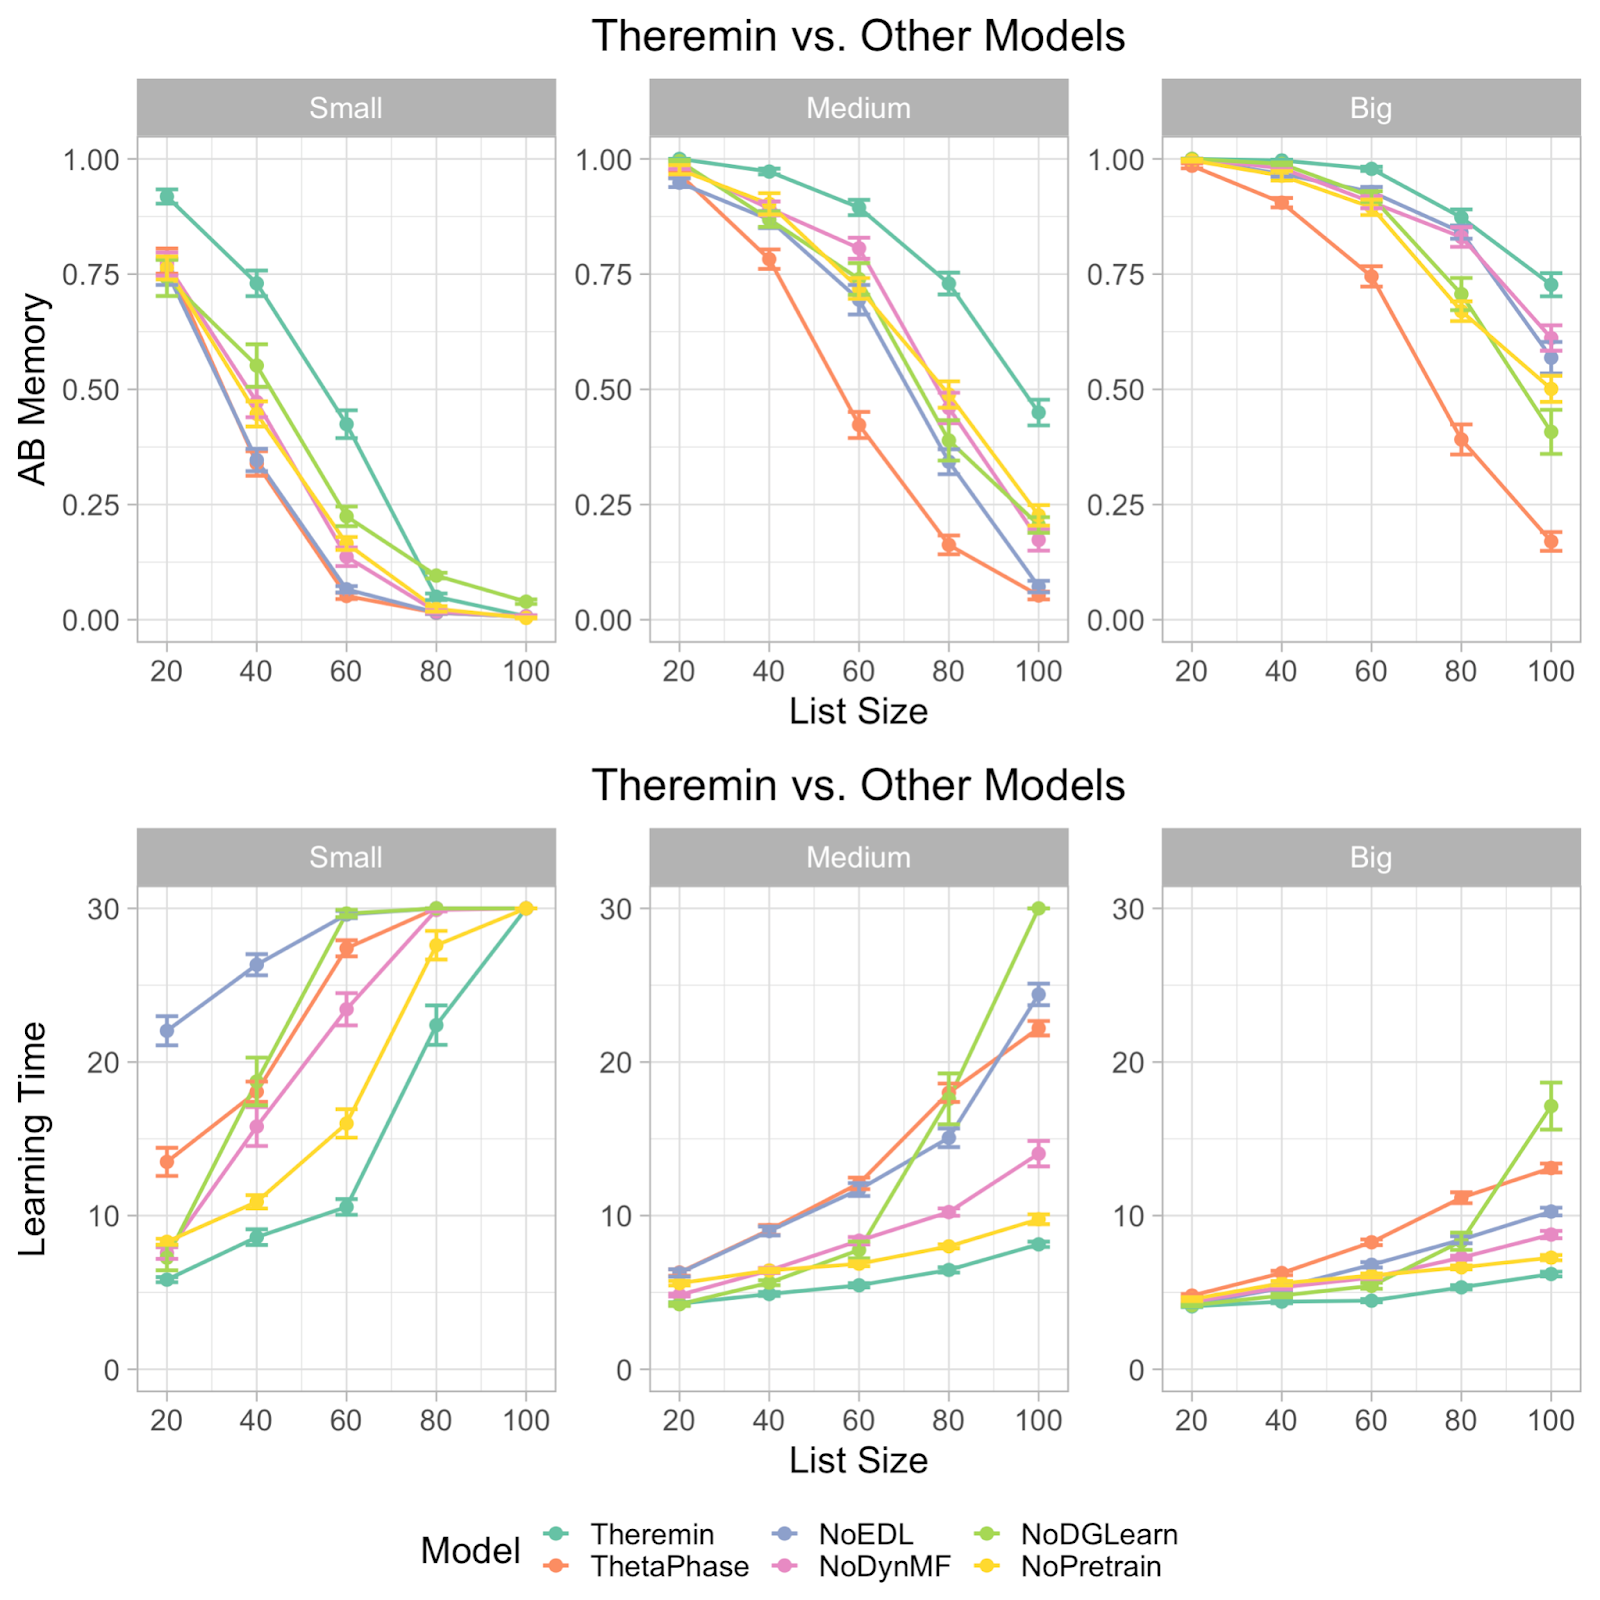
\includegraphics[width=4in]{fig_hip_edl_mods}
  \caption{\footnotesize Theremin vs. other Models on AB memory and learning time. NoEDL is the Theremin without the new error-driven learning mechanism. NoDynMF is the Theremin with same mossy fiber strength during training and testing. NoDGLearn is the Theremin with ECin $\rightarrow$ DG learning off. NoPretrain is the Theremin without pretraining CA1.}
\label{fig.mods}
\end{figure}

To more specifically test the effects of the new error-driven CA3 mechanism in the Theremin model, we directly compared the Theremin model with another Theremin model without error-driven CA3 component (labeled as NoEDL), but with everything else the same. For this and subsequent comparisons, we focus on the medium and large network sizes, as the small case often failed to learn at all for larger list sizes.  Figure~\ref{fig.mods} shows that, except for the smallest list size (20 items), Theremin retained significantly more AB memory (\emph{ps} \textless \ .01, except big network with list size of 20 (\emph{p} = 0.321)) and learned faster (\emph{ps} \textless \ .01, except big network with list size of 20 (\emph{p} = 0.343)) than NoEDL.  Thus, it is clear that this error-driven learning mechanism is responsible for a significant amount of the improved performance of the Theremin model relative to the earlier theta-phase model.

To determine the contributions of the other new mechanisms included in the Theremin model, we compared the full Theremin to versions without each of these mechanisms (Figure~\ref{fig.mods}).  The NoDynMF version eliminated the mechanism of dynamically decreasing the strength of MF inputs from DG to the CA3 during recall, and the results show a significant effect on performance for all but the smallest list size (20 items) (NEpoch \emph{ps} \textless \ .01, except big network with list size of 20 (\emph{p} = .013), ABMem \emph{ps} \textless \ .01, except big network with list size of 20 and 80 (\emph{p} = 0.127)). 

To determine the importance of learning in ECin $\rightarrow$ DG pathway overall, we tested a NoDGLearn variant with no learning at all in this pathway.  In principle, the DG could support its pattern separation function without any learning at all, relying only on the high levels of pattern separation and random PP connectivity.  However, we found that learning in this pathway is indeed important, with an overall decrease in performance for larger list sizes (above 40 items) (NEpoch \emph{ps} \textless \ .01, BigHip List40 \emph{p} = .011; ABMem \emph{ps} \textless \ .01, BigHip List40 \emph{p} = .025).  Interestingly, as the list size scaled up, the NoDGLearn model learned increasingly more slowly, such that it was even slower than the theta-phase model at a list size of 100. This effect is attributable to the strong effect of DG on training the CA3, and when the DG's ability to drive strong pattern separation is compromised, it significantly affects CA3 and thus the overall memory performance.

The higher rate of weight decrease (LTD = long-term depression in biological terms) relative to weight increases in the ECin $\rightarrow$ DG pathway were also important: eliminating this asymmetry significantly decreased performance for larger list sizes (above 60 items) (NEpoch \emph{ps} \textless \ .01, SmallHip List60 \emph{p} = .051; ABMem \emph{ps} \textless \ .05, BigHip List80 \emph{p} = .129).  We also found that a lower learning rate in the ECin $\rightarrow$ DG pathway improved the ABMem score (reducing interference), but resulted in slower learning, and vice-versa for higher learning rates, consistent with the fundamental tradeoff between learning rate and interference that underlies the complementary learning systems framework \citep{McClellandMcNaughtonOReilly95}.  Likewise, due to optimized parameters in Theremin, comparing it to a lower or higher learning rate model would result in significant improvement in ABMem or NEpoch, respectively, but not both. Thus, we compared two Theremin variants that had dramatic differences in both ABMem and NEpoch. Higher learning rate resulted in faster learning (\emph{ps} \textless \ .01) but less ABMem (\emph{ps} \textless \ .01) compared to lower learning rate for list sizes over 40, vice versa.

The final mechanism we tested was the pretraining of the EC $\leftrightarrow$ CA1 encoder pathway, to reflect long-term semantic learning in this pathway.  The NoPretrain variant showed significantly worse performance at all but the smallest list sizes (NEpoch \emph{ps} \textless \ .01; ABMem \emph{ps} \textless \ .05 except BigHip List20 (\emph{p} = .155)). 

\subsection{Representational dynamics}

\begin{figure}
  \centering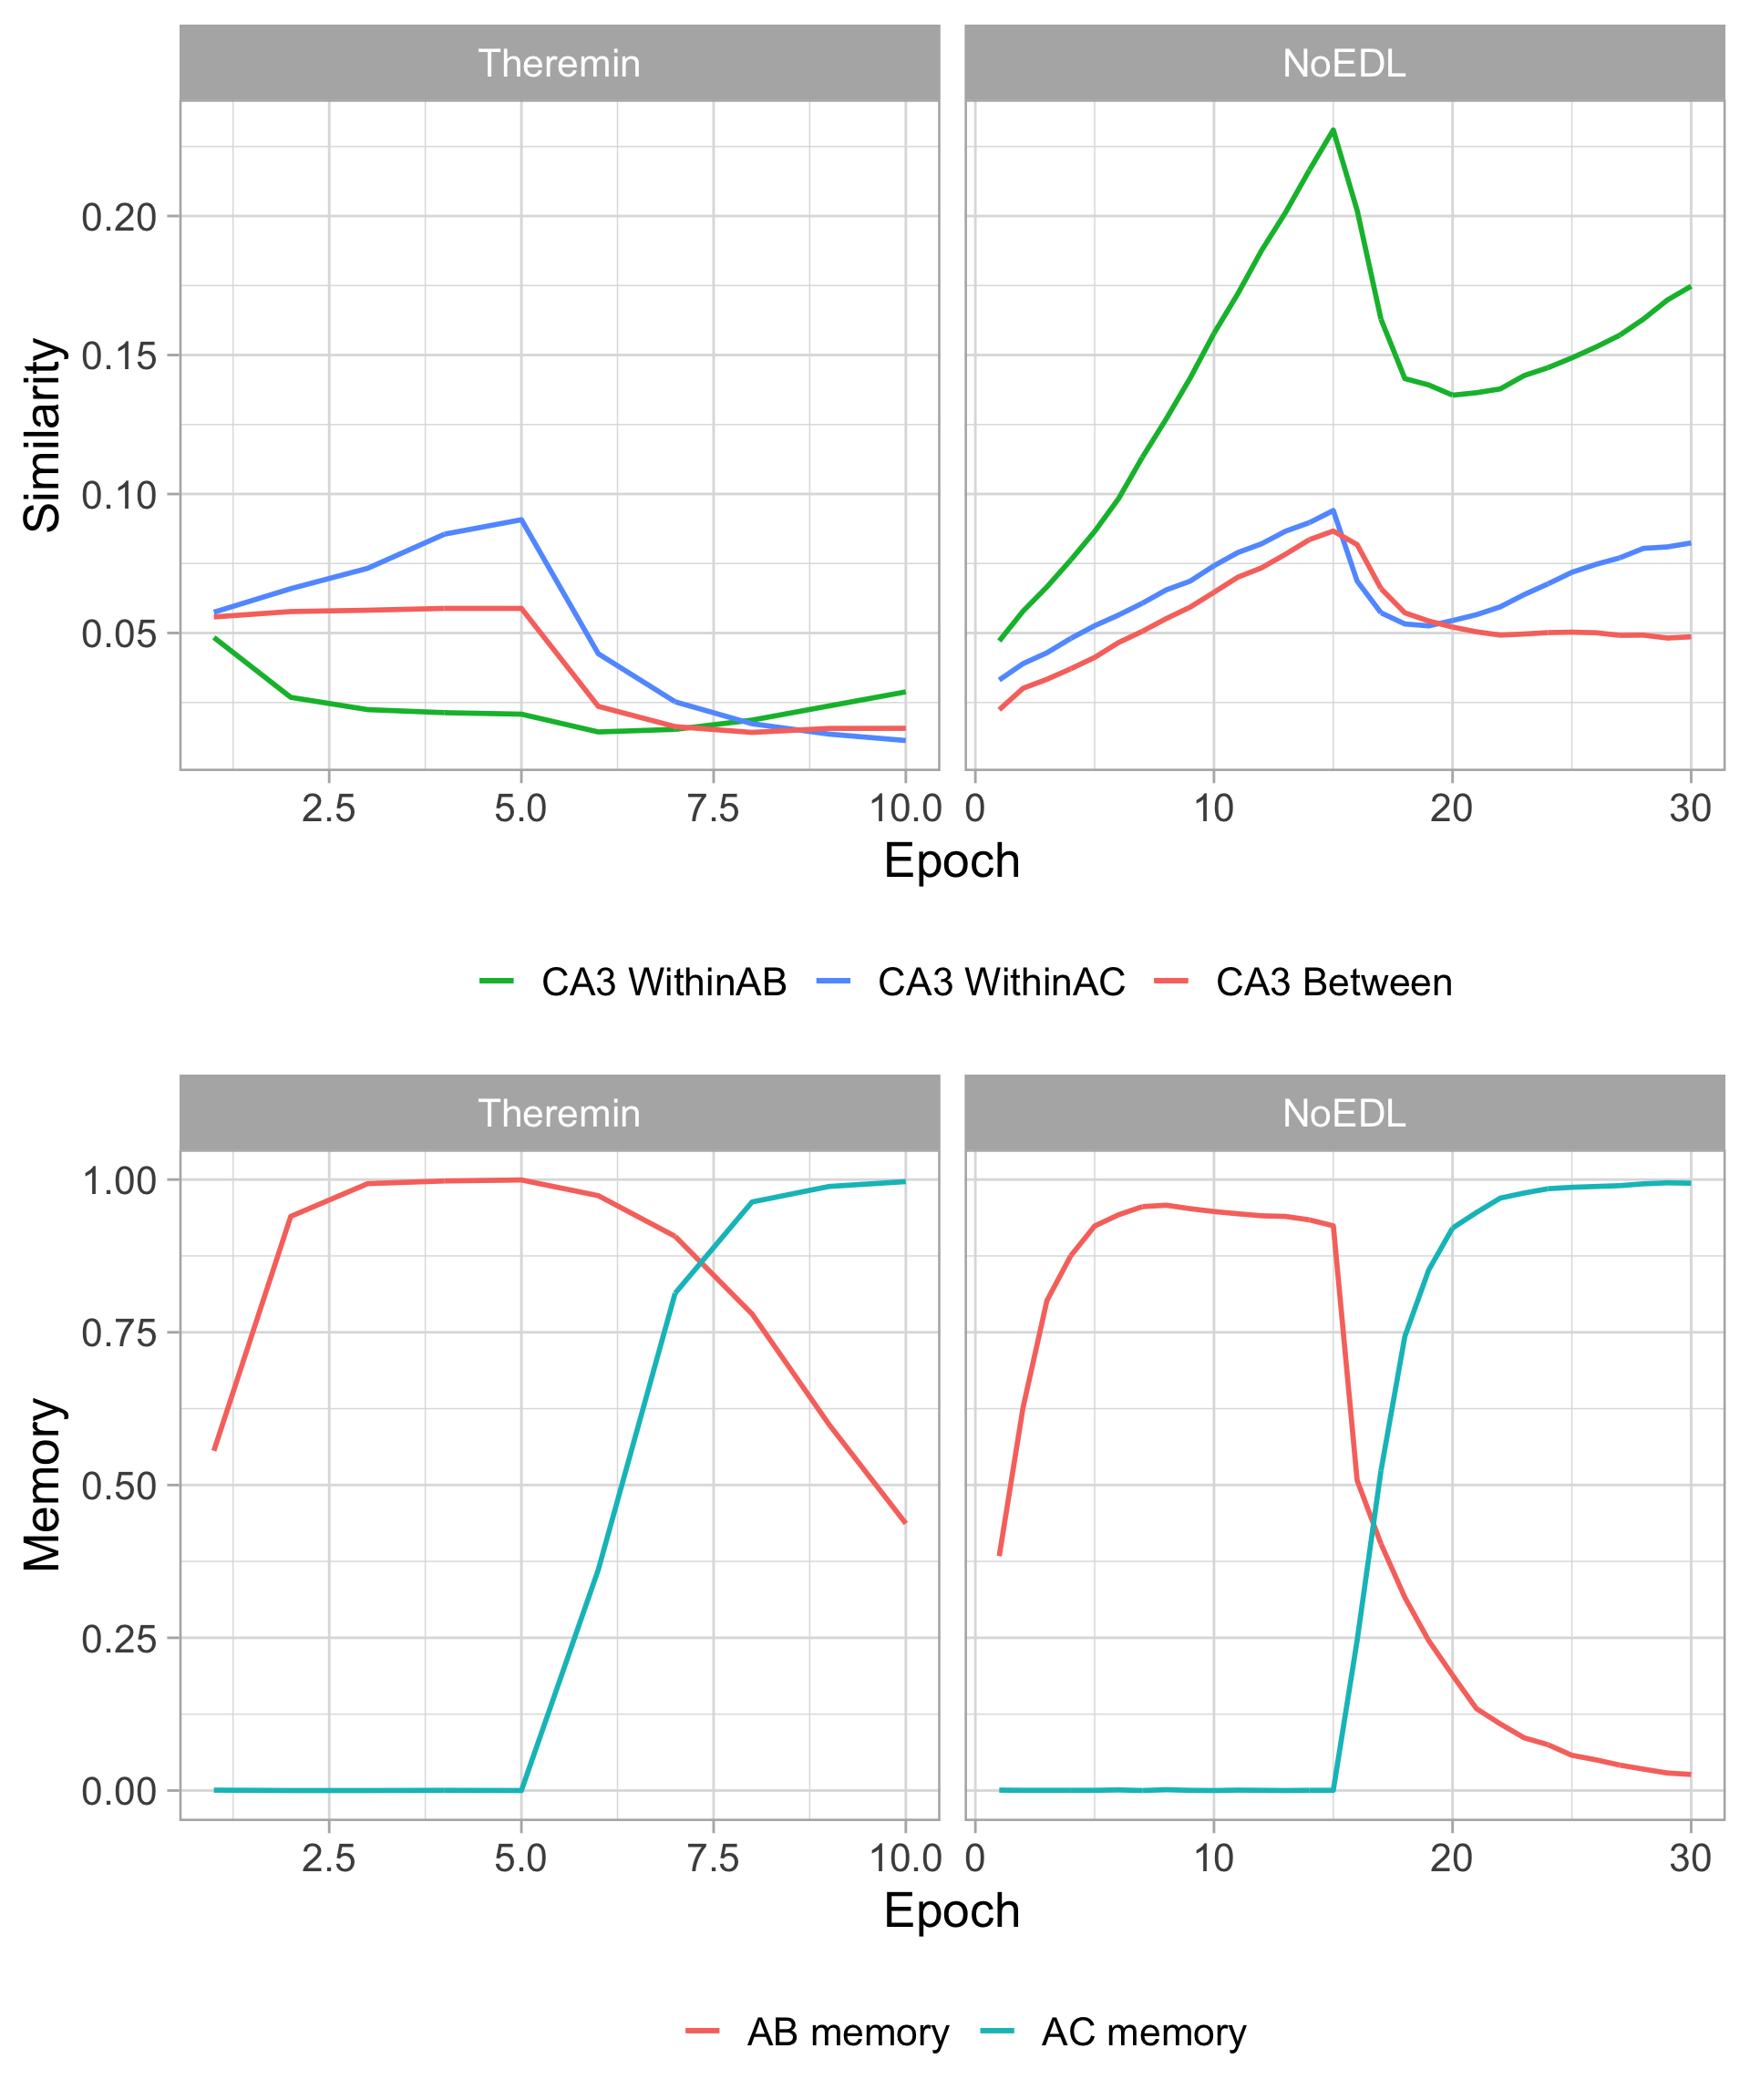
\includegraphics[width=4in]{fig_hip_edl_test_stats}
  \caption{\footnotesize Statistics for area CA3 over the course of testing (List 100, Medium sized network). Representational similarity analyses (RSA) for area CA3 for Theremin vs. NoEDL show how the error-driven learning in Theremin reduces the representational overlap (top left) whereas the Hebbian learning in NoEDL increases the representational overlap (top right).  This explains the differential interference as shown in the AB Memory plot for each case (bottom row). The number of epochs used in Theremin training was set to a fixed number (i.e., 10) that enabled complete learning of AB and AC lists, while in NoEDL was set to the maximum amount used in the current paper (i.e., 30).}
\label{fig.test_stats}
\end{figure}

Having established the basic memory performance effects of the error-driven CA3 and other mechanisms in the Theremin model, we now turn to some analyses of the network representations and dynamics to attempt to understand in greater detail how the error-driven learning shapes representations during learning, how the activation dynamics unfold over the course of the theta cycle within a single trial of learning, and how these dynamics change over multiple iterations of learning.  For these analyses, we focus on the 100-item list size, and the medium sized network, comparing the full Theremin model vs. the NoEDL model, to focus specifically on the effects of error-driven learning in the CA3 pathways.

Figure~\ref{fig.test_stats} shows a representational similarity analysis (RSA) of the different hippocampal layers over the course of learning, comparing the average correlation of representations in CA3 within each list (all AB items and all AC items, e.g., A1B1 vs. A2B2) and between lists (AB vs. AC, e.g., A1B1 vs. A1C1).  These plots also show the proportion of items correctly recalled from each list, with the switch over from the AB to AC list happening half-way through the run (we fixed this crossover point to enable consistent averaging across 30 simulated subjects, using a number of epochs that allowed successful learning for each condition).  These results show that the error-driven learning in the full Theremin model immediately learns to decrease the similarity of representations within the list (e.g., WithinAB when learning AB) and between lists over training, while the Hebbian learning in the NoEDL model fails to separate these representations and results in increases in similarity over time.  This explains the reduced interference and improved learning times for the error-driven learning mechanism, and is consistent with the idea that the continuous weight changes associated with Hebbian learning are deleterious.

\begin{figure}
  \centering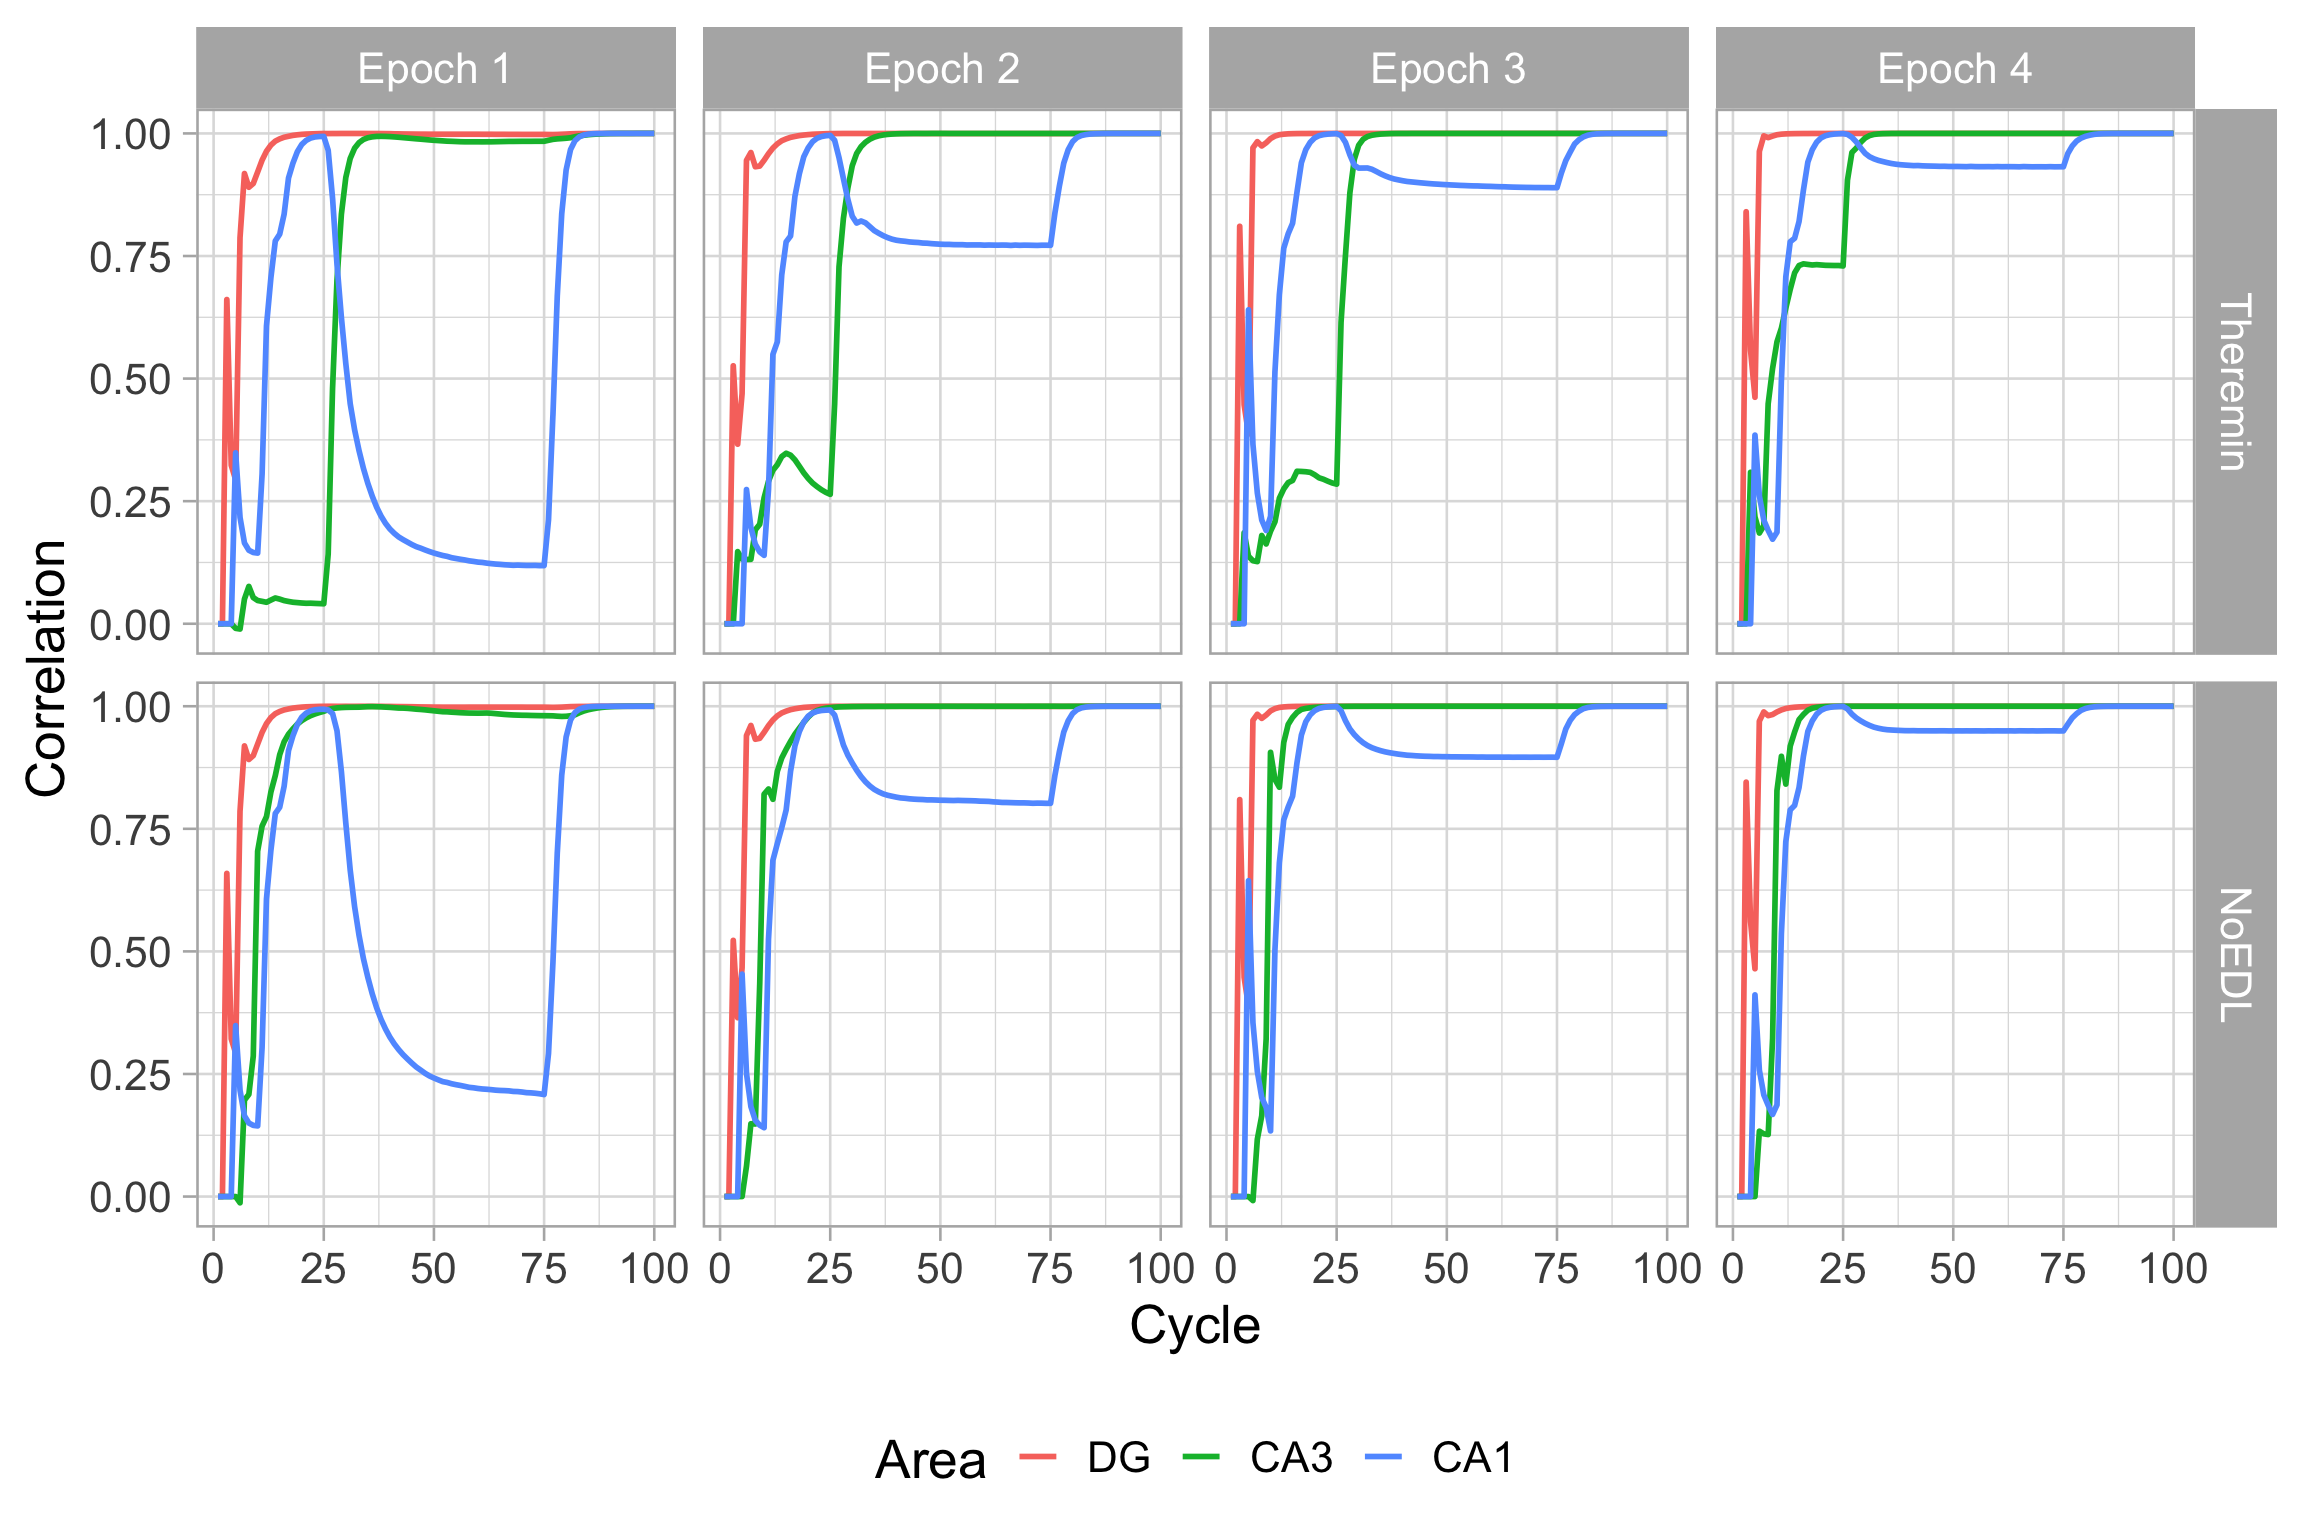
\includegraphics[width=4in]{fig_hip_edl_pat_sim}
  \caption{\footnotesize Changes in hippocampal subregions' pattern similarities over the course of the first 4 epochs of learning, within a full trial for an example AB pair (model timing equivalent to 100 ms), for the Theremin (top row) and NoEDL models (bottom row).  Each line reflects the correlation of the current-time activity pattern relative to the activity pattern at the end of the trial.  Two major effects are evident.  First, the CA1 pattern learns over epochs to quickly converge on the final plus-phase activation state, based on learning in the CA3 $\rightarrow$ CA1 pathway.  Second, the Theremin model shows how the CA3 pattern learns over epochs to converge on the DG-driven activation state that arises after cycle 25, reflecting CA3 error-driven learning.  Additionally, big-loop signals from ECout back to ECin could be observed from cycle 25 to 75 in the first epoch for both models, shifting CA3 patterns slightly off its final patterns.  Drops seen within the first few cycles were due to the settling of temporally different patterns and were not of interest to the current paper.}
\label{fig.pat_sim}
\end{figure}

Figure~\ref{fig.pat_sim} shows an example AB pair plot, with each layer's correlation with the final activation state at the end of the trial across 4 training epochs.  As illustrated in the plot, the learning dynamics in DG, CA3 and CA1 layers follow different learning rules across 4 quarters in one trial.  In the CA3, error-driven learning in the Theremin model causes its activation to converge over the course of learning based on the target DG input that arrives starting after cycle 25.  This learning progression is not evident in the NoEDL model, where Hebbian learning in the CA3 establishes a relatively stable representation early on.  The CA1 shows increasing convergence to the final plus-phase pattern starting in the second and third quarter (cycle 26-75), when CA3 starts to drive CA1.  Interestingly, there is evidence for a ``big-loop'' error signal \citep{KumaranMcClelland12} reflecting activation circulating through the trisynaptic pathway and out through the EC, and back into the  CA3, deviating its pattern from the stabilized one, as depicted by the slightly curved green line in the first epoch.

To elaborate on the error-driven learning dynamics in the Theremin model, as learning progresses, the CA3 pattern in the first quarter becomes increasingly similar to its final pattern (Figure~\ref{fig.pat_sim}). In effect, this similarity signal reflects how close the CA3 pattern is to its final DG-dominated pattern, before DG starts to have an effect on CA3. In the first epoch, CA3 is driven only by ECin $\rightarrow$ CA3 and CA3 $\rightarrow$ CA3 inputs, resulting in a large temporal difference (error signal), which in turn modifies these connections (i.e., heterosynaptic plasticity). This error becomes smaller fast, and learning will stop when there is no more error.  On the other hand, the NoEDL model continually increases the synaptic weights between CA3 and other regions whenever two neurons are active together, according to the Hebbian learning principle.

\section{Discussion}

By incorporating biologically plausible error-driven learning mechanisms at the critical CA3 synapses in our computational model of the hippocampus, along with a few other important optimizations, we have been able to significantly improve learning speed and memory capacity (resistance to interference) compared to our previous model that used Hebbian learning in these synapses. These results demonstrate the critical ability of error-driven learning to automatically limit further learning once it has achieved sufficient changes to support effective memory recall, which then significantly reduces the amount of interference that would otherwise occur from continued synaptic changes.  Furthermore, representational similarity analysis (RSA) was used to illustrate temporal dynamics within the hippocampal formation, which explains the effects of the error-driven learning mechanism, making it possible for the model to make specific subregional predictions that could be tested in experiments.

Another critical contribution of the current model is to specify several biological properties in the hippocampus that could turn into computational benefits. First, turning down DG $\rightarrow$ CA3 strength in recall impairs model performance, presumably due to the need to pattern completion (i.e., CA3 recurrent connections' attractor dynamics) instead of pattern separation (i.e., DG-dominated highly separated patterns). Second, as opposed to the intuitive thinking that DG naturally forms highly separated patterns, no learning in ECin $\rightarrow$ DG pathway is deleterious to model performance, suggesting that there could be more detailed learning dynamics for this pathway to support successful pattern separation. Relevantly, favoring of LTD over LTP is beneficial as it forces DG to form sparse representations, and learning rate in this pathway creates a interference vs. learning time tradeoff that potentially guides the learning efficiency of the hippocampus. Finally, pretraining semantic knowledge of episodic memory components (i.e., representation of items and context) in the EC $\leftrightarrow$ CA1 pathway, is important for the hippocampus to perform effective learning. 

The idea that error-driven learning operates within the hippocampus is consistent with the longstanding idea that the hippocampus acts as a comparator \citep{Gray82,Vinogradova01,LismanGrace05}.  These theories focused on the idea that the hippocampus generates one single scalar value error signal as a function of the relative mismatch between a predicted state and the actual next state (e.g., novelty), which is then used to guide actions.  For example \citet{Gray82} proposed that combining previous sensory information and the motor plan creates predictions about the current state, which are then compared with the actual current sensory information.  The motor plan is maintained if the two states match, but stopped and attempts to solve the problem posed if there is a mismatch.  By contrast, our model uses internally-generated error signals between the DG and CA3 to drive rapid episodic encoding of the current state, consistent with the classical model of overall hippocampal function as an episodic memory system. 

Another computational model of hippocampal function directly employed backpropagation for error-driven learning \citep{MyersGluck95}.  In this model, the hippocampal network is a predictive autoencoder, which learns to regenerate the input patterns and predict future reinforcement.  The cortical network representations are shaped by hippocampal training signals and output a behavioral response such as an anticipatory reflex.  Simulations with this model and its hippocampus-lesioned variant have been shown to replicate a wide range of conditioned behaviors in rats and rabbits \citep{GluckMyers93}.  However, it is still unclear how backpropagation could work in the brain biologically.

One promising idea about how backpropagation could work biologically is using local information in the form of neural activities from different time points or spatial compartments, which in some cases follow the gradient produced by backpropagation \citep{LillicrapSantoroMarrisEtAl20, OReilly96}.  Multiple lines of hippocampal studies point to realization of such a temporal-difference form of error-driven learning in the hippocampus, which contributes to its key cognitive functions.  

First, the idea that the hippocampus is important for prediction is central to a number of related sequence learning models \citep{Levy96,WallensteinHasselmo97,JensenLisman96,TsodyksSkaggsSejnowskiEtAl96,Rolls13,SchapiroTurk-BrowneBotvinickEtAl17}. In these models, the recurrent connections in area CA3 learn to associate prior time step representations with subsequent time step patterns, thus learning to predict the current state based on the previous state.  Unlike the above comparator models, these sequence learning models are not just driving a summary scalar prediction-error signal, but rather is learning a high-dimensional prediction about how the state evolves over time.  This use of prediction error within the hippocampus is not mutually exclusive with the error-driven learning for episodic memory in our model, and we will explore ways of integrating these two perspectives in future work.  In particular, we have been investigating the potential for error-driven predictive learning in posterior cortex \citep{OReillyRussinZolfagharEtAl21}, and similar mechanisms may be operating, potentially at longer time scales, in the hippocampus.

Second, local neural activation signals can drive the nonmonotonic plasticity learning dynamics explored by Norman and colleagues \citep{RitvoTurk-BrowneNorman19}.  Specifically, using external inputs as teaching signals, the model contrasts a prediction phase (given input and activity spread, the final activity pattern at the output layer) and an outcome phase (correct answers are presented to the network) to perform supervised learning in the hippocampus.  Together with unsupervised learning, this model achieves powerful nonmonotonic learning curve, such that pattern differentiation or integration occurs depending on the activation level of memories.

Finally, combining the current hippocampal model with a neocortex offers a convincing computational account for testing effect, such that testing generates better memory compared to restudy \citep{LiuO'ReillyRanganath21}.  Using the same temporal difference error-driven learning mechanism and the CLS framework, the fast-learning hippocampus teaches the slow-learning neocortex to produce more precise answers based on the error between different patterns generated by only neocortex and both neocortex and hippocampus.  Indeed, these models share the same fundamental temporal-difference driven learning rule, and mainly differ in the sources of the temporal differences that drive it.  

In summary, we argue here that hippocampus models benefit from the temporal difference error-driven learning mechanisms, such that memory capacity and learning speed could be dramatically improved, and a wide range of learning and memory phenomenon could be explained computationally.  These mechanisms could emerge naturally out of neurophysiological properties of the hippocampal circuits beyonds CA1 \citep{KetzMorkondaOReilly13} and CA3 without referring to backpropagation.  More importantly, we advocate the idea of combining error-driven learning in the hippocampus with the longstanding Hebbian learning to achieve higher biological validity.  The presented Theremin model offers a powerful hippocampal framework that could be used to test against specific experimental results and to coordinate with other cortical regions computationally for generating novel predictions.

\section{Deleted Discussion (leave it here for now)}

One consideration is whether the improved learning exhibited by the Theremin model is now somehow at a superhuman level, and thus renders our model less plausible as a realistic model of hippocampal function.  However, there are several factors mitigating against this concern.  First, our models are trained and tested in a ``blank slate'' manner, with no prior episodic memories that would likely drive significant proactive interference (note that the pretraining is only done on the EC $\leftrightarrow$ CA1 pathway, and not on the overall episodic memory circuitry involving CA3).  

In addition, these granule cells have been identified as a rare locus of adult neurogenesis \citep{neurogenesis}, which has been shown to enhance the pattern separation capacity of the DG in computational models \citep{Becker}.  A future version of the model will explore the effects of neurogenesis, and other speculative possible feedback circuits within the DG as discussed later.

Results revealed that the new CA3-focused error-driven learning mechanism could improve model performance by comparing CA3 states from different time points to generate error signals for training synaptic weights.  However, is better performance correct performance? 

There are also a few directions for a further error-driven hippocampal learning system based on neurophysiological evidence.  For example, there is evidence that CA3 pyramidal cells might also backpropagate to mossy cells in the polymorphic layer of DG, which could potentially form errors to train DG representations (cites).  Another possible error source is the big-loop recurrence that plays a critical role in the hippocampal system, supporting integration of information from neocortex across different episodes (Koster et al., 2018; Kumaran, Hassabis, McClelland, 2016). Although not directly studied in the current paper, the big-loop error could still be observed in the model (Figure~\ref{fig.pat_sim}) and might be another type of temporal difference error signals that trains the hippocampus. 

In the current model, we broaden the use of this kind of error-driven learning mechanism in the hippocampus as suggested by our previous version of the model \citep{KetzMorkondaOReilly13} and suggest that the hippocampus should break its historical affiliation with Hebbian learning. 

Interestingly, Schapiro and colleagues have recently discovered that the error-driven learning dynamics of the theta-phase based monosynaptic EC $\leftrightarrow$ CA1 pathway support a form of statistical learning, that was previously thought to only exist in more purely cortical areas \citep{SchapiroTurk-BrowneBotvinickEtAl17}.  Likewise, adopting an error-driven learning framework for the trisynaptic pathway opens up further opportunities for powerful error-driven learning phenomena in this pathway, and the hippocampal system as a whole.

\section{Appendix}

\subsection{Model Parameters}

Size params
Key params
Number of units in each subfield


\bibliography{ccnlab}
% use: bibexport -o hip_edl.bib hip_edl_2021.aux to regenerate:
%\bibliography{hip_edl}

\end{document}
